\documentclass[letterpaper,addpoints,answers]{exam}
\usepackage{graphicx}
\usepackage{multicol}
\usepackage{wrapfig}
\usepackage{tikz}

\usetikzlibrary{calc}

\makeatletter
\def\grd@save@target#1{%
  \def\grd@target{#1}}
\def\grd@save@start#1{%
  \def\grd@start{#1}}
\tikzset{
  grid with coordinates/.style={
    to path={%
      \pgfextra{%
        \edef\grd@@target{(\tikztotarget)}%
        \tikz@scan@one@point\grd@save@target\grd@@target\relax
        \edef\grd@@start{(\tikztostart)}%
        \tikz@scan@one@point\grd@save@start\grd@@start\relax
        \draw[minor help lines] (\tikztostart) grid (\tikztotarget);
        \draw[major help lines] (\tikztostart) grid (\tikztotarget);
        \grd@start
        \pgfmathsetmacro{\grd@xa}{\the\pgf@x/1cm}
        \pgfmathsetmacro{\grd@ya}{\the\pgf@y/1cm}
        \grd@target
        \pgfmathsetmacro{\grd@xb}{\the\pgf@x/1cm}
        \pgfmathsetmacro{\grd@yb}{\the\pgf@y/1cm}
        \pgfmathsetmacro{\grd@xc}{\grd@xa + \pgfkeysvalueof{/tikz/grid with coordinates/major step x}}
        \pgfmathsetmacro{\grd@yc}{\grd@ya + \pgfkeysvalueof{/tikz/grid with coordinates/major step y}}
        \foreach \x in {\grd@xa,\grd@xc,...,\grd@xb}
        \node[anchor=north] at (\x,\grd@ya) {\pgfmathprintnumber{\x}};
        \foreach \y in {\grd@ya,\grd@yc,...,\grd@yb}
        \node[anchor=east] at (\grd@xa,\y) {\pgfmathprintnumber{\y}};
      }
    }
  },
  minor help lines/.style={
    help lines,
    gray,
    line cap =round,
    xstep=\pgfkeysvalueof{/tikz/grid with coordinates/minor step x},
    ystep=\pgfkeysvalueof{/tikz/grid with coordinates/minor step y}
  },
  major help lines/.style={
    help lines,
    line cap =round,
    line width=\pgfkeysvalueof{/tikz/grid with coordinates/major line width},
    xstep=\pgfkeysvalueof{/tikz/grid with coordinates/major step x},
    ystep=\pgfkeysvalueof{/tikz/grid with coordinates/major step y}
  },
  grid with coordinates/.cd,
  minor step x/.initial=.5,
  minor step y/.initial=.2,
  major step x/.initial=1,
  major step y/.initial=1,
  major line width/.initial=1pt,
}
\makeatother

\tikzset{
    right angle quadrant/.code={
        \pgfmathsetmacro\quadranta{{1,1,-1,-1}[#1-1]}     % Arrays for selecting quadrant
        \pgfmathsetmacro\quadrantb{{1,-1,-1,1}[#1-1]}},
    right angle quadrant=1, % Make sure it is set, even if not called explicitly
    right angle length/.code={\def\rightanglelength{#1}},   % Length of symbol
    right angle length=2ex, % Make sure it is set...
    right angle symbol/.style n args={3}{
        insert path={
            let \p0 = ($(#1)!(#3)!(#2)$) in     % Intersection
                let \p1 = ($(\p0)!\quadranta*\rightanglelength!(#3)$), % Point on base line
                \p2 = ($(\p0)!\quadrantb*\rightanglelength!(#2)$) in % Point on perpendicular line
                let \p3 = ($(\p1)+(\p2)-(\p0)$) in  % Corner point of symbol
            (\p1) -- (\p3) -- (\p2)
        }
    }
}


\graphicspath{{final/}}

\begin{document}

\begin{coverpages}
 \large\bfseries
 
 \noindent 
 Physics 107: Physics for Life-Sciences

 \vspace{2ex}
 \noindent
 Final Exam: December 15, 2015

 \vspace{3ex}
 \noindent 
 This test is administered under the rules and regulations of the honor code of the College of William \& Mary.

 \vspace{2ex}
 \noindent 
 Name:\enspace\makebox[2.3in]{\hrulefill} \\

 \noindent 
 Signature:\enspace\makebox[2in]{\hrulefill} \\

 \vspace{5ex}
 \noindent 
 Instructions:
 \begin{itemize}
  \item This is a closed book, closed notes test.
  \item Calculators are NOT needed and NOT allowed. Devices with wireless connections are NOT allowed.
  \item Start your work from the fundamental equations on the formula sheet, and derive any additional expressions that you may need.
  \item Circle your answer for each part of each problem. 
  \item Clearly mark out any work that you wish the grader to disregard.  Do not waste your time erasing.
  \item Your work will be graded based on your ability to write down a logical and organized solution grounded in the correct assessment of the physics of a situation. No credit will be given for an answer that is not justified by a logical solution or where that justification is not organized or readable. Partial credit will be given up to the point where your solution departs from a correct analysis of the physics involved for any given part of a problem.
 \end{itemize}

 \pagebreak

 \begin{center}
  \gradetable[v][questions]
 \end{center}
 
\end{coverpages}
 

\begin{questions}

\printanswers

% 5 multiple choice questions

\begin{question}[5]
\begin{multicols}{2}
A car drives with a constant speed over a circularly shaped hill and into a circularly shaped valley, both with radius $R$. Which one of the following statements about the normal forces on the car is true? The normal force in point A is denoted as $N_A$, the normal force in point B as $N_B$, and the weight of the car as $W$.
\begin{center}
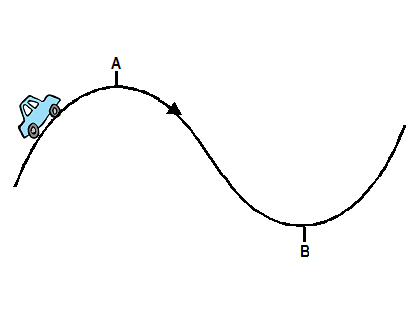
\includegraphics[width=0.28\textwidth]{car_hill}
\end{center}
\end{multicols}
\begin{checkboxes}
 \choice $N_A = N_B = W$: The normal forces on the car at point A and point B are both equal to the weight of the car.
 \choice $N_A > W > N_B$: The normal force on the car will be larger than the weight of the car at point A, but smaller than the weight at point B.
 \correctchoice $N_B > W > N_A$: The normal force on the car will be larger than the weight of the car at point B, but smaller than the weight at point A.
 \choice $N_A > N_B > W$: The normal force on the car will be larger at point A than at point B, and both will be larger than the weight of the car.
 \choice $N_B > N_A > W$: The normal force on the car will be larger at point B than at point A, and both will be larger than the weight of the car.
\end{checkboxes}
\end{question}

\begin{question}[5]
\begin{multicols}{2}
A 1-kg rock is suspended by a massless string from one end of a measuring stick with a length of 1\,m. What is the weight of the measuring stick if it is balanced by a support force at the 0.25\,m mark?
\begin{center}
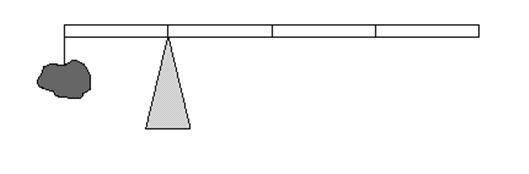
\includegraphics[width=0.4\textwidth]{rock_balance}
\end{center}
\end{multicols}
\begin{checkboxes}
 \choice 0.25\,kg
 \choice 0.5\,kg
 \correctchoice 1\,kg
 \choice 2\,kg
 \choice Impossible to determine.
\end{checkboxes}
\end{question}

\begin{question}[5]
\begin{multicols}{2}
A mass on a spring is describing simple harmonic motion. The position of the mass as a function of time is shown in the figure. At the time corresponding to point $P$, which one of the following statements is true?
\begin{center}
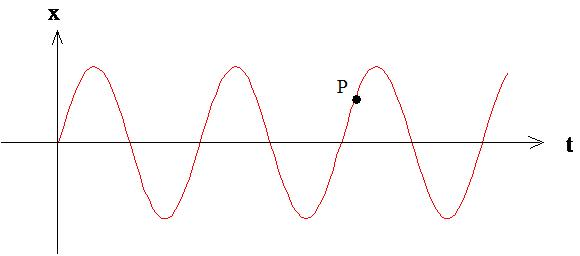
\includegraphics[width=0.35\textwidth]{oscillation}
\end{center}
\end{multicols}
\begin{checkboxes}
 \correctchoice The velocity $v$ is greater than 0 and the acceleration $a$ is less than 0.
 \choice The velocity $v$ is less than 0 and the acceleration $a$ is greater than 0.
 \choice The velocity $v$ is greater than 0 and the acceleration $a$ is greater than 0.
 \choice The velocity $v$ is less than 0 and the acceleration $a$ is less than 0.
 \choice The velocity $v$ and acceleration $a$ are both 0.
\end{checkboxes}
\end{question}

\pagebreak

\begin{question}[5]
\begin{multicols}{2}
Three waves are traveling along identical strings. Wave B has twice the amplitude of the other two. Wave C has half the wavelength of waves A or B.

Which wave has the higher frequency?
\begin{checkboxes}
 \choice A has the highest frequency.
 \choice B has the highest frequency.
 \correctchoice C has the highest frequency.
 \choice A and B both have the highest frequency.
 \choice A and C both have the highest frequency.
\end{checkboxes}
\begin{center}
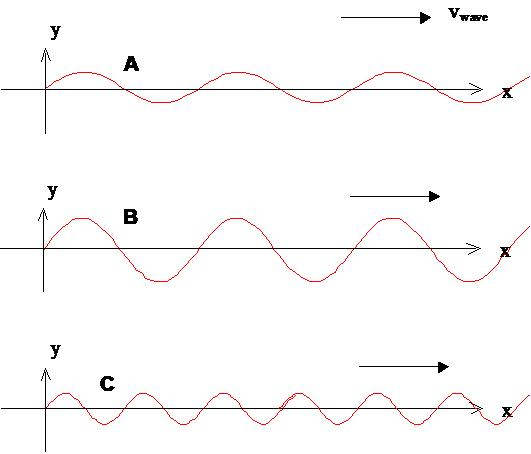
\includegraphics[width=0.35\textwidth]{waves}
\end{center}
\end{multicols}
\end{question}

\begin{question}
Consider the ballistic pendulum shown in the figure. This is an example of a perfectly inelastic collision in which both masses stick together after the collision. The mass $M$ is 5 times larger than the mass $m$.
\begin{center}
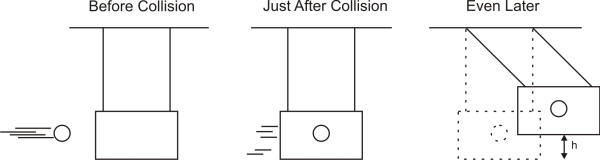
\includegraphics[width=0.4\textwidth]{ballistic_pendulum}
\end{center}
\begin{parts}
\part[5] What was the speed of the combined mass $M + m$ just after its collision?
\begin{checkboxes}
 \choice $v = v_0$
 \choice $v = v_0/2$
 \choice $v = 2v_0/3$
 \choice $v = v_0/5$
 \correctchoice $v = v_0/6$
\end{checkboxes}
\part[5] Which one of the following statements is correct for the collision and subsequent motion of the pendulum?
\begin{checkboxes}
 \choice Momentum is always conserved, and mechanical energy is conserved because this is an inelastic collision.
 \choice All initial kinetic energy of $m$ is converted into gravitational potential energy of $M + m$.
 \choice The pendulum will have constant angular velocity since no torque is exerted by the string.
 \correctchoice Only momentum is conserved during the collision, and mechanical energy is conserved at all times except during the collision.
 \choice The angle $\theta$ at the highest point will be larger if the length $L$ of the pendulum is larger.
\end{checkboxes}
\end{parts}
\end{question}

\pagebreak

\begin{question}
A woman with a mass $m$ of 50.0\,kg is doing push-ups, as shown in the figure below. In addition to her weight, she is supported by the force at her toes and her hands. \textit{Note:} You may approximate the magnitude of the gravitational acceleration $g$ as $10.0\,\mbox{m}/\mbox{s}^2$.
\begin{center}
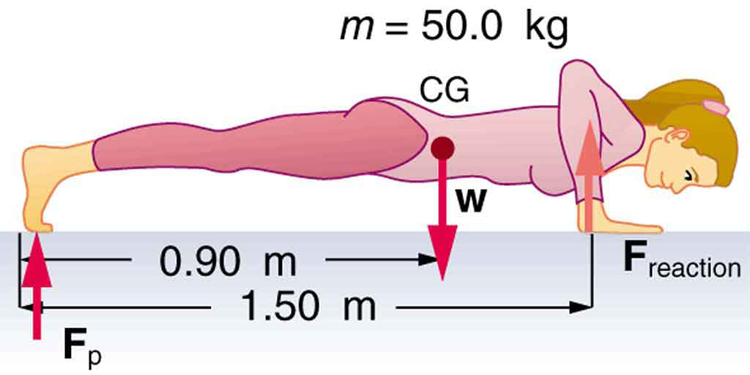
\includegraphics[width=0.5\textwidth]{push_ups}
\end{center}
\begin{parts}
\part[5] Assume that the woman holds her position for a brief moment during the push-ups. What is the force that the woman exerts on the floor with \textit{each} hand?
\begin{solution}[1.5in]
We use the torque equation, $\tau_{net} = 0$, with the pivot point at her feet. We find that $\tau_{net} = 1.50\,\mbox{m} \cdot F_{reaction} - 0.90\,\mbox{m} \cdot 50\,\mbox{kg} \cdot 10\,\mbox{m}/\mbox{s}^2 = 0$. This means that $F_{reaction} = 300$\,N, or each hand exerts a force of 150\,N.
\end{solution}
\part[5] What is the force that the woman exerts on the floor with \textit{each} foot?
\begin{solution}[1.25in]
We use the net force equation, $F_{net} = F_p + F_{reaction} - W = 0$. This immediately results in $F_p = 200$\,N, or each foot exerts a force of 100\,N.
\end{solution}
\part[5] How much work does she do if her center of mass rises by 20\,cm?
\begin{solution}[1.25in]
The change in gravitational potential energy is $m g h$ or 100\,J.
\end{solution}
\part[5] What is her useful power output if she does 30 push-ups in one minute? Assume she does only work when pushing up, not when lowering herself again.
\begin{solution}[1.25in]
If she does 30 push-ups per minute, that's 2 seconds per push-up. The power output is then 100\,J per 2\,s or 50\,W.
\end{solution}
\end{parts}
\end{question}

\pagebreak

\begin{question}
\begin{multicols}{2}
As shown in the figure, the object $m_1 = 1.0$\,kg starts at an initial height $h_{1i} = 1.0$\,m and with an initial speed $v_{1i} = 4.0$\,m/s, swings downward and strikes (in an elastic collision) object $m_2 = 2$\,kg which is initially at rest. \textit{Note:} You may approximate the magnitude of the gravitational acceleration $g$ as $10.0\,\mbox{m}/\mbox{s}^2$.
\begin{center}
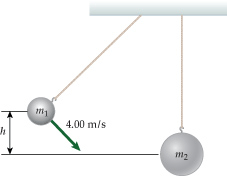
\includegraphics[width=0.3\textwidth]{pendulum_collision}
\end{center}
\end{multicols}
\begin{parts}
 \part[10] What is the speed $v_1$ of $m_1$ just before the collision?
 \begin{solution}[2in]
  The sum of the initial kinetic and potential energy is $KE + PE = \frac{1}{2} m_1 v_{1i}^2 + m_1 g h$. With the information given this is $\frac{1}{2} (1\,\mbox{kg}) (4.0\,\mbox{m}/\mbox{s})^2 + (1\,\mbox{kg}) (10\,\mbox{m}/\mbox{s}^2) (1\,\mbox{m}) = 8\,\mbox{J} + 10\,\mbox{J} = 18\,\mbox{J}$. This energy is converted into kinetic energy, $\frac{1}{2} m_1 v_1^2 = 18\,\mbox{J}$, with $v_1 = 6\,\mbox{m}/\mbox{s}$.
 \end{solution}
 \part[10] What is the velocity of $m_1$ and what is the velocity of $m_2$ just after the elastic collision? Give both magnitude and direction. Assume that the positive direction is to the right. \textit{Note:} At a cost of 1 point, use a speed of $m_1$ of 9\,m/s just before the collision if you are not confident in your answer above.
 \begin{solution}[2in]
  We use the two equations $v_1 - v_2 = v'_2 - v'_1$ and $m_1 v_1 + m_2 v_2 = m_1 v'_1 + m_2 v'_2$ to determine the velocity of $m_1$ just after the collision: $$v'_1 = \frac{m_1 - m_2}{m_1 + m_2} v_1 = \frac{-1\,\mbox{kg}}{3\,\mbox{kg}} 6\,\mbox{m}/\mbox{s} = -2\,\mbox{m}/\mbox{s}.$$ The velocity of $m_2$ is then $v'_2 = v_1 + v'_1 = 4\,\mbox{m}/\mbox{s}$.
  
  The alternative solution was $v'_1 = -3\,\mbox{m}/\mbox{s}$ and $v'_2 = 6\,\mbox{m}/\mbox{s}$.
 \end{solution}
 \part[5] To what height does $m_2$ swing after the collision? \textit{Note:} At a cost of 1 point, use a speed of $m_2$ just after the collision of 6\,m/s if you are not confident in your answer above.
 \begin{solution}[1in]
  The kinetic energy $\frac{1}{2} m_2 (v'_2)^2$ of $m_2$ is converted into potential energy $m_2 g h_2$, with a height given by $$h_2 = \frac{(v'_2)^2}{2 g} = \frac{16}{20}\,\mbox{m} = 0.8\,\mbox{m}.$$ The alternative solution was $h_2 = 1.8\,\mbox{m}$.
 \end{solution}
\end{parts}
\end{question}

\pagebreak

\begin{question}
\begin{multicols}{2}
A fire hose has a diameter of 8.0\,cm. The hose goes up a ladder to a nozzle with an inside diameter of 4.0\,cm at a height of 10.0\,m. The water flows out of the nozzle with a speed of 40\,m/s. The water has a density of $1000\,\mbox{kg}/\mbox{m}^3$ and a viscosity of $1.00\,\mbox{mPa}\cdot\mbox{s}$.
\begin{center}
 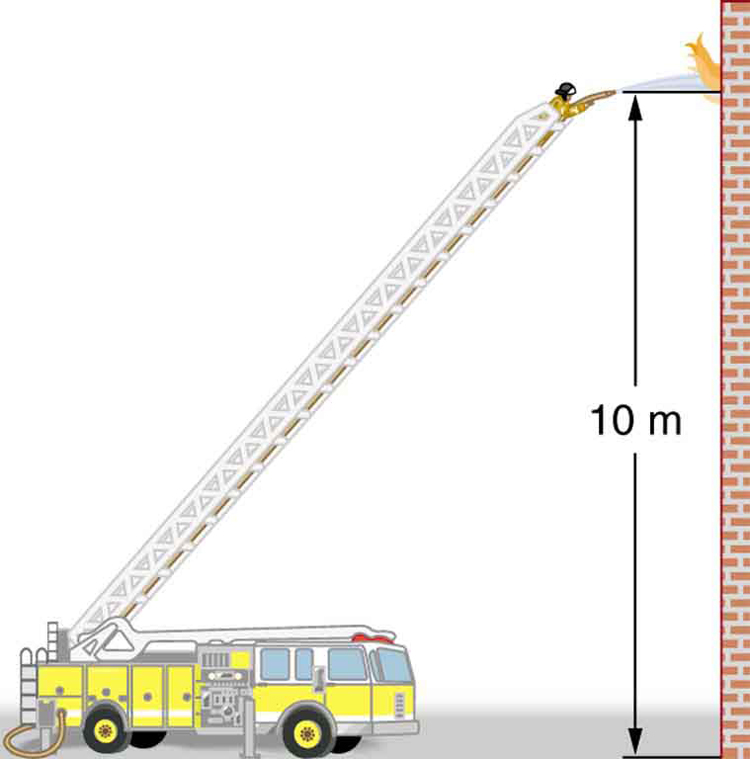
\includegraphics[width=0.3\textwidth]{firehose}
\end{center}
\end{multicols}
\begin{parts}
 \part[5] What is the velocity with which the water will flow through the hose as it leaves the fire engine pumps at ground level?
 \begin{solution}[1.5in]
  Due to the continuity equation $A_{hose} v_{hose} = A_{nozzle} v_{nozzle}$, which will mean that $v_{hose} = \frac{1}{4} v_{nozzle} = 10\,\mbox{m}/\mbox{s}$.
 \end{solution}
 \part[5] Will the flow in the nozzle be turbulent?
 \begin{solution}[1.5in]
  We determine the Reynolds number for the nozzle: $$N_R = \frac{2 \rho v r}{\eta} = \frac{2 \cdot 1000\,\mbox{kg}/\mbox{m}^3 \cdot 10\,\mbox{m}/\mbox{s} \cdot 0.04\,\mbox{m}}{10^{-3}\,\mbox{Pa}\cdot\mbox{s}} = 800,000.$$ This is higher than 3000, so the flow will indeed be turbulent.
 \end{solution}
 \part[5] What must the gauge pressure in the fire engine be to sustain this flow? Gauge pressure is the overpressure relative to atmospheric pressure.
 \begin{solution}[2in]
  We use Bernoulli's law to determine the pressure difference $P_{hose} - P_{atm}$, which is equal to 
  $$P_{hose} - P_{atm} = P_{hose} - P_{nozzle} = \rho g h + \frac{1}{2} \rho v_{nozzle}^2 - \frac{1}{2} \rho v_{hose}^2 = \rho g h + \frac{1}{2} \rho (v_{nozzle}^2 - v_{hose}^2).$$
  After plugging in the values found earlier, we get
  $$P_{hose} - P_{atm} = 1000\,\mbox{kg}/\mbox{m}^3 \cdot 10\,\mbox{m}/\mbox{s}^2 \cdot 10\,\mbox{m} + \frac{1}{2} 1000\,\mbox{kg}/\mbox{m}^3 \left( \left(40\,\mbox{m}/\mbox{s}\right)^2 - \left(10\,\mbox{m}/\mbox{s}\right)^2 \right) = 850,000\,\mbox{Pa}.$$
 \end{solution}
\end{parts}
\end{question}

\pagebreak

\begin{question}
A large housefly 5.0 meters away from you makes a noise of 30\,dB.
\begin{parts}
 \part[5] How many decibels would the housefly make if it were 50 centimeters away?
 \begin{solution}[1.5in]
  If the fly is 10 times closer, the noise will be 10\,dB louder, so 40\,dB.
 \end{solution}
 \part[5] With a noise level of 30\,dB, how much energy falls on your eardrum in one minute, which you can assume as a square surface of 1.0\,cm by 1.0\,cm?
 \begin{solution}[1.5in]
  A noise level of 30\,dB corresponds to an intensity that is $10^3$ times higher than the threshold of hearing $I_0$, or $I = 10^{-9}\,\mbox{W}/\mbox{m}^2$. The power arriving on your eardrum with a surface area $A = 10^{-4}\,\mbox{m}^2$ is then $P = I A = 10^{-13}\,\mbox{W}$. The energy deposited during a 60 second interval is then $E = 60 \cdot 10^{-13}$\,J.
 \end{solution}
\end{parts}
\end{question}

\begin{question}
% variables
\newcommand{\dopplerfhornsrc}{990}
\newcommand{\dopplerfbellsrc}{1000}
\newcommand{\dopplervtrain}{10}
\newcommand{\dopplerfhornobs}{\the\numexpr \dopplerfhornsrc*100/(100-\dopplervtrain) \relax}
\newcommand{\dopplerfhornobsaway}{\the\numexpr \dopplerfhornsrc*100/(100+\dopplervtrain) \relax}
\newcommand{\dopplerfbellobs}{\the\numexpr \dopplerfbellsrc*(100+\dopplervtrain)/100 \relax}
\newcommand{\dopplerfbellobsaway}{\the\numexpr \dopplerfbellsrc*(100-\dopplervtrain)/100 \relax}
A train is approaching a railroad crossing. On the train a horn is sounding with a frequency of \dopplerfhornsrc\,Hz. The railroad crossing has a warning bell which is ringing with a frequency of \dopplerfbellsrc\,Hz.
\begin{parts}
\part[5] The engineer on the approaching train hears the warning bell at the railroad crossing with a higher frequency of \dopplerfbellobs\,Hz. What is the speed of the train, expressed as a fraction of the speed of sound $v$? For example, $0.\dopplervtrain \cdot v$ for a train moving at \dopplervtrain\% of the speed of sound, or approximately 75\,mph.
\begin{solution}[2in]
We are in the case of a observer moving towards the source (the engineer on the approaching train towards the railroad crossing). The relevant formula is $$f_{obs} = f_{src} \frac{v + v_{obs}}{v} = f_{src} \left(1 + \frac{v_{obs}}{v}\right)$$ from which we want to determine $v_{obs}$. We find that $$v_{obs} = \left(\frac{f_{obs}}{f_{src}} - 1\right)\cdot v = \left(\frac{\dopplerfbellobs}{\dopplerfbellsrc} - 1\right) \cdot v = 0.\dopplervtrain \cdot v.$$
\end{solution}
\part[5] With the speed of the train that you found in the previous part, what is the frequency with which the railroad crossing attendant hears the horn of the approaching train? \textit{Note:} Use a speed of the train that is 10\% of the speed of sound if you are not confident in your answer above.
\begin{solution}[2in]
Now we are in the case of a source moving towards the observer (the attendant at the railroad crossing). The relevant formula is $$f_{obs} = f_{src} \frac{v}{v - v_{src}} = \dopplerfhornsrc\,\mbox{Hz} \frac{v}{v - 0.\dopplervtrain \cdot v} = \dopplerfhornsrc\,\mbox{Hz} \frac{1}{0.9} = \dopplerfhornobs\,\mbox{Hz}.$$
\end{solution}
\part[5] After the train passes the railroad crossing what is now the frequency with which the engineer on the train hears the warning bell at the railroad crossing?
\begin{solution}[2in]
Now we are in the case of a observer moving away from the source (the engineer on the train moving away from the railroad crossing). The relevant formula is $$f_{obs} = f_{src} \frac{v - v_{obs}}{v} = f_{src} \left(1 - \frac{v_{obs}}{v}\right) = \dopplerfbellsrc\,\mbox{Hz} \left(1 - \frac{0.\dopplervtrain \cdot v}{v}\right) = \dopplerfbellobsaway\,\mbox{Hz}.$$
\end{solution}
\part[5] After the train passes the railroad crossing what is now the frequency with which the railroad crossing attendant hears the horn on the train as it is moving away?
\begin{solution}[2in]
Now we are in the case of a stationary observer with a source that is moving away. The relevant formula is $$f_{obs} = f_{src} \frac{v}{v + v_{src}} = \dopplerfhornsrc\,\mbox{Hz} \frac{v}{v + 0.\dopplervtrain \cdot v} = \dopplerfhornobsaway\,\mbox{Hz}.$$
\end{solution}
\end{parts}
\end{question}

\end{questions}

 \pagebreak

 {\small Nothing to see here, please move along.} \\

 \pagebreak
 
 {\Large Possibly useful relations (feel free to detach this page):}
  
% Test 1
%  \fontseries{\seriesdefault}
%  \begin{multicols}{2}
%  \Large
%  \noindent
%  $\vec{v}_{avg} = \Delta\vec{x} / \Delta t$ \\
%  $x = x_0 + v_0 t + \frac{1}{2} a t^2$ \\
%  $v^2 = v_0^2 + 2 a (x - x_0)$ \\
%  $R = \frac{v_0^2}{g}\sin 2\theta$ \\
%  $\vec{F}_{net} = m \vec{a}$ \\
%  $\vec{W} = m \vec{g}$ \\
%  $\cos\theta = \hbox{adjacent}/\hbox{hypotenuse}$ \\
%  $\sin\theta = \hbox{opposite}/\hbox{hypotenuse}$ \\
%  $\sin 30^\circ = \cos 60^\circ = \frac{1}{2}$ \\
%  $\cos 30^\circ = \sin 60^\circ = \frac{\sqrt{3}}{2}$ \\
 
%  \noindent
%  $\vec{a}_{avg} = \Delta\vec{v} / \Delta t$ \\
%  $v = v_0 + a t$ \\
%  $v_{avg} = \frac{v_0 + v}{2}$ \\
%  $h = \frac{v_0^2}{2 g} \sin^2 \theta$ \\
%  $\vec{F}_{BA} = - \vec{F}_{AB}$ \\
%  $\vec{g} = 9.80\,m/s^2$ downward \\
%  $x = \frac{-b \pm \sqrt{b^2 - 4 a c}}{2 a}$ \\
%  $\tan\theta = \sin\theta / \cos\theta$ \\
%  $\tan 45^\circ = 1$ \\
%  \end{multicols}


% Test 2
%  \fontseries{\seriesdefault}
%  \begin{multicols}{2}
%  \Large
%  \noindent
%  $\vec{v}_{avg} = \Delta\vec{x} / \Delta t$ \\
%  $\vec{a}_{avg} = \Delta\vec{v} / \Delta t$ \\
%  $x = x_0 + v_0 t + \frac{1}{2} a t^2$ \\
%  $v = v_0 + a t$ \\
%  $v_{avg} = \frac{v_0 + v}{2}$ \\
%  $v^2 = v_0^2 + 2 a (x - x_0)$ \\
%  $\vec{F}_{net} = m \vec{a}$ \\
%  $\vec{F}_{BA} = - \vec{F}_{AB}$ \\
%  $W = F d \cos\theta$ \\
%  $W_{net} = -\Delta PE = \Delta KE$ \\
%  $KE = \frac{1}{2} m v^2$ \\
%  $PE_k = \frac{1}{2} k x^2$ \\
%  $PE_g = m g h$ \\
%  $KE_i + PE_i + W_{nc} = KE_f + PE_f$ \\
%  $P = \frac{W}{\Delta t}$ \\
%  $\hbox{Eff} = \frac{W_{out}}{E_{in}}$ \\
%  $\cos\theta = \hbox{adjacent}/\hbox{hypotenuse}$ \\
%  $\sin\theta = \hbox{opposite}/\hbox{hypotenuse}$ \\
%  $\tan\theta = \sin\theta / \cos\theta$ \\
%  $\sin 30^\circ = \cos 60^\circ = \frac{1}{2}$ \\
%  $\cos 30^\circ = \sin 60^\circ = \frac{\sqrt{3}}{2}$ \\
%  $\tan 45^\circ = 1$ \\

%  \noindent
%  $R = \frac{v_0^2}{g}\sin 2\theta$ \\
%  $h = \frac{v_0^2}{2 g} \sin^2 \theta$ \\
%  $0 \le f_s \le \mu_s N$ \\
%  $f_k = \mu_k N$ \\
%  $\frac{F}{A} = Y \frac{\Delta L}{L}$ \\
%  $F_k = -k x$ \\
%  $\vec{W} = m \vec{g}$ \\
%  $\vec{g} = 9.80\,\mbox{m}/\mbox{s}^2$ downward \\
%  $F_G = G \frac{m M}{r^2}$ \\
%  $G = 6.67 \times 10^{-11}\,\mbox{N}\cdot\mbox{m}^2/\mbox{kg}^2$ \\
%  $\vec{I} = \vec{F}_{avg} \Delta t$ \\
%  $\vec{p} = m \vec{v}$ \\
%  $\vec{F}_{net} = \frac{\Delta \vec{p}}{\Delta t}$ \\
%  $v_1 - v_2 = v'_2 - v'_1$ \\
%  $\theta = \frac{s}{r}$ \\
%  $v = r \omega$ \\
%  $f = \frac{1}{T}$ and $\omega = 2 \pi f = \frac{2 \pi}{T}$ \\
%  $a_c = \frac{v^2}{r} = r \omega^2$ \\
%  $F_c = m\frac{v^2}{r} = m r \omega^2$ \\
%  $1\,\hbox{cal} = 4.186$\,J and $1\,\hbox{Cal} = 1000$\,cal \\ 
%  $x = \frac{-b \pm \sqrt{b^2 - 4 a c}}{2 a}$ \\
%  \end{multicols}


% Test 3
 \fontseries{\seriesdefault}
 \begin{multicols}{2}
 \normalsize
 \noindent
 $\vec{v}_{avg} = \Delta\vec{x} / \Delta t$ \\
 $\vec{a}_{avg} = \Delta\vec{v} / \Delta t$ \\
 $x = x_0 + v_0 t + \frac{1}{2} a t^2$ \\
 $v = v_0 + a t$ \\
 $v_{avg} = \frac{v_0 + v}{2}$ \\
 $v^2 = v_0^2 + 2 a (x - x_0)$ \\
 $\vec{F}_{net} = m \vec{a}$ \\
 $\vec{F}_{BA} = - \vec{F}_{AB}$ \\
 $W = F d \cos\theta$ \\
 $W_{net} = -\Delta PE = \Delta KE$ \\
 $P = \frac{W}{\Delta t}$ \\
 $\hbox{Eff} = \frac{W_{out}}{E_{in}}$ \\
 $KE_i + PE_i + W_{nc} = KE_f + PE_f$ \\
 $PE_k = \frac{1}{2} k x^2$ \\
 $PE_g = m g h$ \\
 $KE_{trans} = \frac{1}{2} m v^2$ \\
 $KE_{rot} = \frac{1}{2} I \omega^2$ \\
 $I_{point} = M R^2$ \\
 $I_{disk} = \frac{1}{2} M R^2$ \\
 $I_{sphere} = \frac{2}{5} M R^2$ \\
 $P = \frac{F}{A}$ \\
 $P_{gauge} = P - P_{atm}$ \\
 $\rho = \frac{M}{V}$ \\
 $\rho_{water} = 10^3\,\hbox{kg}/\hbox{m}^3$ \\
 $Q = \frac{\Delta V}{\Delta t} = A v$ \\
 $Q = \frac{\Delta P \pi r^4}{8 \eta L}$ \\
 $\hbox{Power} = P Q$ \\
 $A \cdot v = \hbox{constant}$ \\
 $P + \rho g y + \frac{1}{2} \rho v^2 = \hbox{constant}$ \\
 $F_B = \rho g V_{displaced}$ \\
 $F_{ST} = \gamma L$ \\
 $P = \frac{4 \gamma}{r}$ \\
 $h = \frac{2 \gamma \cos\theta}{\rho g r}$ \\
 $N_R = \frac{\rho v L}{\eta} = \frac{2 \rho v r}{\eta}$ \\
 $x_{rms} = \sqrt{2 D t}$ \\
 $f_{obs} = f_{src} \frac{v}{v \pm v_{src}}$ with $-$ for src moving towards obs \\
 $f_{obs} = f_{src} \frac{v \pm v_{obs}}{v}$ with $+$ for obs moving towards src \\
 $f_{beat} = |f_1 - f_2|$ \\
 $\cos\theta = \hbox{adjacent}/\hbox{hypotenuse}$ \\
 $\sin\theta = \hbox{opposite}/\hbox{hypotenuse}$ \\
 $\tan\theta = \sin\theta / \cos\theta$ \\
 $\sin 30^\circ = \cos 60^\circ = \frac{1}{2}$ \\
 $\cos 30^\circ = \sin 60^\circ = \frac{\sqrt{3}}{2}$ \\
 $\tan 45^\circ = 1$ \\
 $x = \frac{-b \pm \sqrt{b^2 - 4 a c}}{2 a}$ \\

 \noindent
 $R = \frac{v_0^2}{g}\sin 2\theta$ \\
 $h = \frac{v_0^2}{2 g} \sin^2 \theta$ \\
 $0 \le f_s \le \mu_s N$ \\
 $f_k = \mu_k N$ \\
 $\frac{F}{A} = Y \frac{\Delta L}{L}$ \\
 $F_k = -k x$ \\
 $\vec{W} = m \vec{g}$ \\
 $\vec{g} = 9.80\,\mbox{m}/\mbox{s}^2$ downward \\
 $F_G = G \frac{m M}{r^2}$ \\
 $G = 6.67 \times 10^{-11}\,\mbox{N}\cdot\mbox{m}^2/\mbox{kg}^2$ \\
 $\vec{I} = \vec{F}_{avg} \Delta t$ \\
 $\vec{p} = m \vec{v}$ \\
 $\vec{F}_{net} = \frac{\Delta \vec{p}}{\Delta t}$ \\
 $v_1 - v_2 = v'_2 - v'_1$ \\
 $\theta = \frac{s}{r}$ \\
 $v = r \omega$ \\
 $f = \frac{1}{T}$ and $\omega = 2 \pi f = \frac{2 \pi}{T}$ \\
 $a_c = \frac{v^2}{r} = r \omega^2$ \\
 $F_c = m\frac{v^2}{r} = m r \omega^2$ \\
 $\tau = r F \sin\theta = r_\perp F$ \\
 $\omega = \frac{\Delta \theta}{\Delta t}$ \\
 $\alpha = \frac{\Delta \omega}{\Delta t}$ \\
 $\tau = I \alpha$ \\
 $L = I \omega$ \\
 $\tau = \frac{\Delta L}{\Delta t}$ \\
 $x(t) = A \cos \omega t$ and $x_{max} = A$ \\
 $v(t) = - A \omega \sin \omega t$ and $v_{max} = A \omega$ \\
 $a(t) = - A \omega^2 \cos \omega t$ and $a_{max} = A \omega^2$ \\
 $E = \frac{1}{2} k x^2 + \frac{1}{2} m v^2 = \frac{1}{2} k x_{max}^2 = \frac{1}{2} m v_{max}^2$ \\
 $v = \sqrt{T/\mu}$ with $\mu = \frac{m}{L}$ \\
 spring: $\omega = \sqrt{k/m}$ \\
 pendulum: $\omega = \sqrt{g/\ell}$ \\
 $y(x,t) = A \cos (\omega t \pm k x)$ with $-$ for left-moving wave \\
 $\omega = \frac{2 \pi}{T}$ and $k = \frac{2 \pi}{\lambda}$ \\
 $v = \lambda f = \frac{\omega}{k}$ \\
 $v_{sound} = 331\,\hbox{m/s} \sqrt{\frac{T}{273\,K}}$ \\
 string: $\lambda_n = \frac{2 L}{n}$, $f_n = \frac{n v}{2 L}$ with $n = 1,2,3,\ldots$ \\
 open-open: $\lambda_n = \frac{2 L}{n}$, $f_n = \frac{n v}{2 L}$ with $n = 1,2,3,\ldots$ \\
 open-closed: $\lambda_n = \frac{4 L}{n}$, $f_n = \frac{n v}{4 L}$ with $n = 1,3,5,\ldots$ \\
 $I = \frac{P}{A} = \frac{P}{4 \pi r^2}$ \\
 $\beta = 10 \log \frac{I}{I_0}$ in dB with $I_0 = 10^{-12}$\,W/m$^2$ \\
 $1\,\hbox{atm} = 10^5\,\hbox{Pa} = 760\,\hbox{mm}\cdot\hbox{Hg}$ \\
 $1\,\hbox{cal} = 4.186$\,J and $1\,\hbox{Cal} = 1000$\,cal \\ 
 \end{multicols}

\end{document}
